\begin{figure}[H]
    \centering
    \includegraphics[width=\textwidth]{figures/cellot-methods/Bunne_Supp_Fig1.png}
    \caption{Predicted and observed marginals of cells profiled by 4i, treated with Imatinib. All extracted intensity and morphology features are shown.}
    \label{supp_fig:4i_all_marginals_imatinib}
\end{figure}

\begin{figure}[H]
    \centering
    \includegraphics[width=\textwidth]{figures/cellot-methods/Bunne_Supp_Fig2.png}
    \caption{Predicted and observed marginals of cells profiled by 4i treated with Trametinib. All extracted intensity and morphology features are shown.}
    \label{supp_fig:4i_all_marginals_trametinib}
 \end{figure}
 
 \begin{figure}[H]
    \centering
    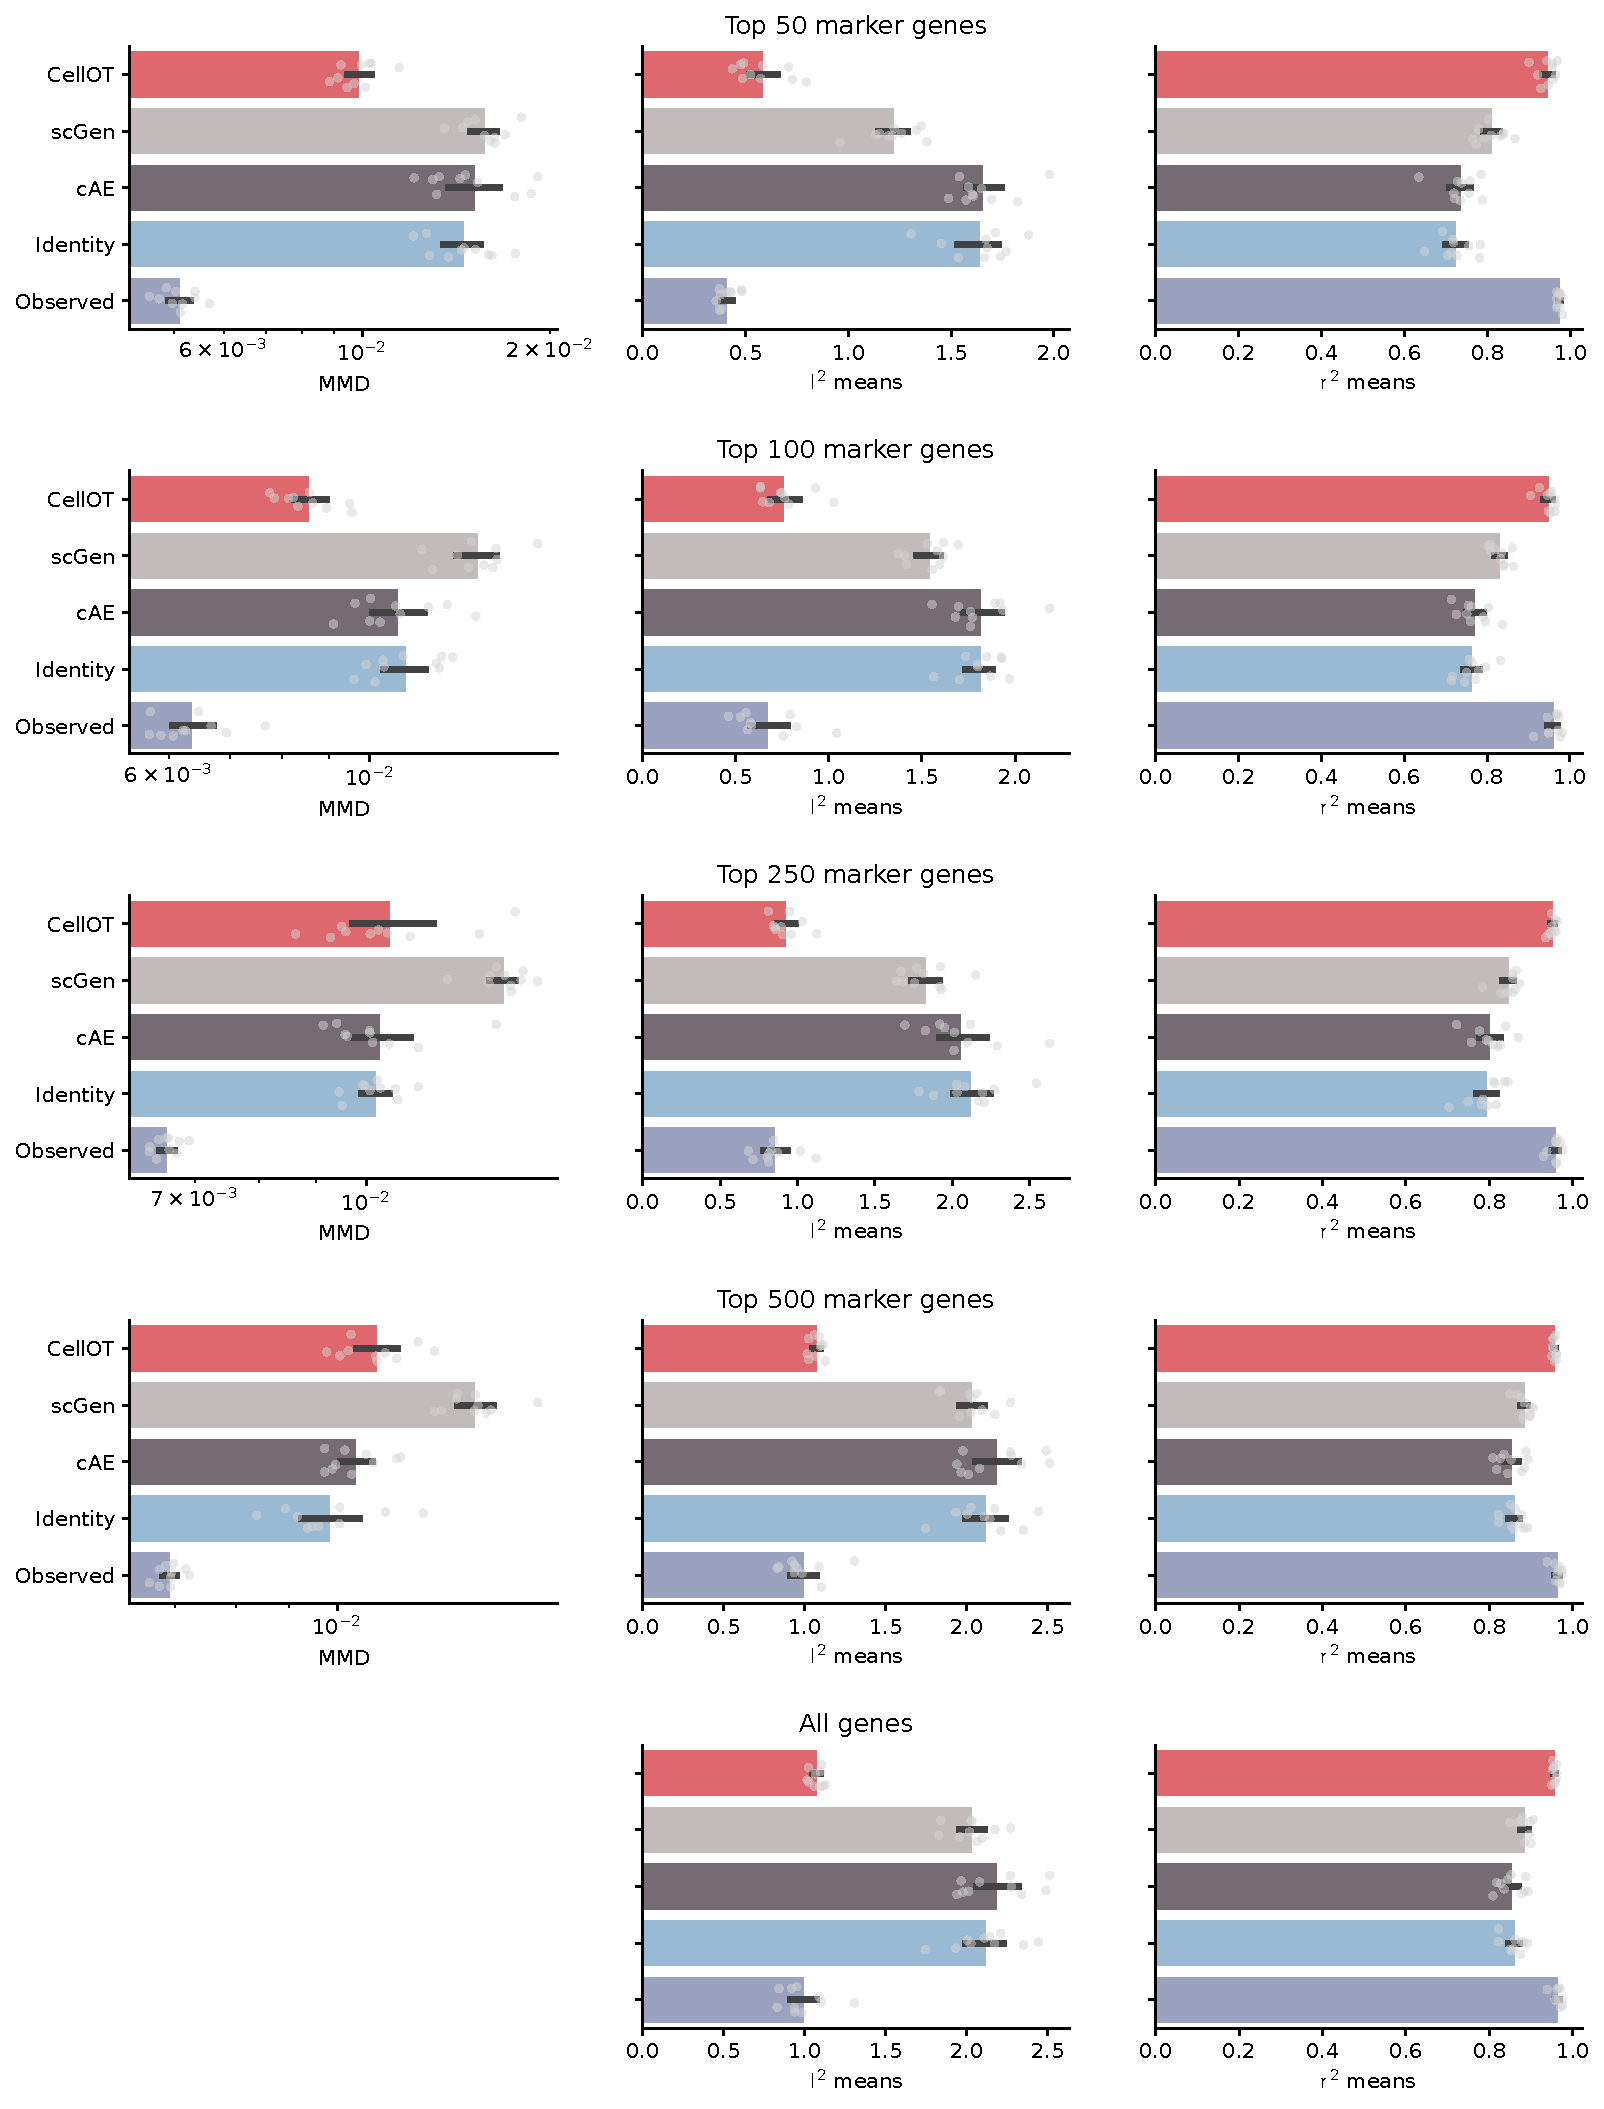
\includegraphics[width=0.9\textwidth]{figures/cellot-methods/Bunne_Supp_Fig7.pdf}
    \caption{Results for single-cell responses for Trametinib the SciPlex3 dataset for different metrics computed on 50, 100, 250, and 500 marker genes, including MMD, $\ell_2$ feature means, and $r^2$ correlation feature means for \textsc{CellOT} as well as different baselines. With increasing dimensionality, the MMD computation is biased. Data is presented as the mean +/- standard deviation across n=10 bootstraps of the test set.}
    \label{supp_fig:sciplex_num_markers}
\end{figure}

\begin{figure}[H]
    \centering
    \includegraphics[width=\textwidth]{figures/cellot-methods/Bunne_Supp_Fig5_p1.pdf}
\end{figure}
\begin{figure}[H]
    \centering
    \includegraphics[width=\textwidth]{figures/cellot-methods/Bunne_Supp_Fig5_p2.pdf}
    \caption{Results on other drugs for the 4i dataset for different metrics, including MMD, $\ell_2$ feature means, and $r^2$ correlation feature means for \textsc{CellOT} as well as different baselines. Data is presented as the mean +/- standard deviation across n=10 bootstraps of the test set.}
    \label{supp_fig:4i_all_results}
\end{figure}

\begin{figure}[H]
    \centering
    \includegraphics[width=.8\textwidth]{figures/cellot-methods/Bunne_Supp_Fig6.pdf}
    \caption{Results on other drugs for the SciPlex 3 dataset for different metrics, including MMD, $\ell_2$ feature means, and $r^2$ correlation feature means for \textsc{CellOT} as well as different baselines. Data is presented as the mean  +/- standard deviation across n=10 bootstraps of the test set.}
    \label{supp_fig:sciplex_all_results}
\end{figure}

\begin{figure}[H]
    \centering
    \includegraphics[width=\textwidth]{./figures/cellot-methods/Bunne_ED_Fig1.pdf}
    \caption{Analysis of dataset structures for the 4i dataset (\textbf{a}, \textbf{b}) and the SciPlex 3 dataset (\textbf{c}). $\textbf{a)}$ Spearman correlations between all feature pairs computed in 4i control cells (bottom) and Sorafenib-treated cells (top). Row colors show the mean value of each feature in control cells and column colors show the effect of the drug on each feature as computed by the difference in means between control and treated. Correlations that changed the most under the perturbation are highlighted in blue. $\textbf{b)}$ Density plot of feature correlations in the control setting vs. treated setting for all 35 4i treatments. Sorafenib values (corresponding to elements in $\textbf{b}$) are scattered above and light blue points correspond to blue boxes in $\textbf{b}$. $\textbf{c)}$ Feature correlation between in the control setting vs. treated setting for all cancer drugs of the SciPlex 3 dataset.}
    \label{supp_fig:data_correlation}
\end{figure}

\begin{figure}[H]
    \centering
    \includegraphics[width=\textwidth]{./figures/cellot-methods/Bunne_ED_Fig2.pdf}
    \caption{Visualization of the learned vector field describing the perturbation response on the single-cell level for \textbf{a)} Dabrafenib, \textbf{b)} Everolimus, and \textbf{c)} Trametinib of the 4i dataset for \textsc{CellOT}, the average effect, and \textsc{scGen} on the first two principal components. Cellular responses are computed as the predicted treated state minus the observed control state for each individual cell. Arrow tails are placed in a grid within PC space and arrow heads correspond to the average response of cells within each neighborhood, projected into PC space.}
    \label{supp_fig:4i_vector_fields}
\end{figure}

\begin{figure}[H]
    \centering
    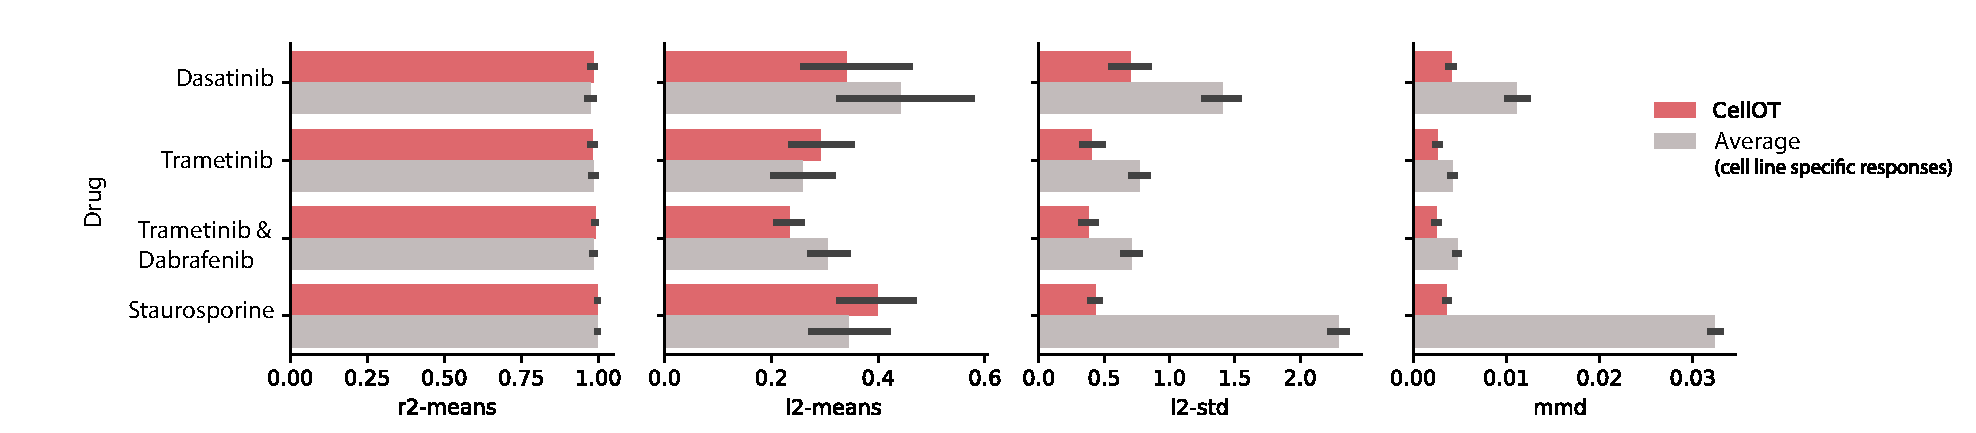
\includegraphics[width=1.05\textwidth]{figures/cellot-methods/Bunne_Supp_Fig13.pdf}
    \caption{Results of predicting perturbation effects of a selection of cancer drugs on 4i data using \textsc{CellOT} and a baseline that predict the average perturbation effect of each cell line (\textsc{Average}). Contrary to \textsc{CellOT}, the baseline requires cell typing, and annotation might not always be trivial. For example, in this setting, cell type markers are affected by the perturbation itself. The benchmark is conducted w.r.t. different metrics, including MMD, $r^2$ correlation feature means, $\ell_2$ feature means, and standard deviation. Data are presented as the mean +/- standard deviation across n=15 bootstraps of the test set.}
    \label{supp_fig:comparison_cellot_average}
\end{figure}

\begin{figure}[b!]
    \centering
    \includegraphics[width=0.95\textwidth]{./figures/cellot-methods/Bunne_ED_Fig3.pdf}
    \caption{(caption next page)}
    \label{supp_fig:4i_analysis_extended}
\end{figure}
\addtocounter{figure}{-1}
\begin{figure}[t!]
\caption{\textbf{a)} High similarity of measured and CellOT-predicted single-cell pERK (phosphor ERK1/2) values at the single-cell level. Scatter plots compares the relationship between measured pERK values of cells (left) treated with Midostaurin (green dots), Palbociclib (blue dots), Panobinostat (red dots), and MLN2480 (purple dots) or (right) predicted for those drugs along the horizontal axis to their corresponding 3NN cells on the vertical axis. For details on the generation of 3NN data, see Online Methods. X mark, square, inverted triangle, and circle represent the mean of the respective measurements per drug. The dashed gray line indicates the diagonal along which the measurements would correlate perfectly. \textbf{b)} The high similarity of measured and CellOT-predicted single-cell pERK (phosphor ERK1/2) values at the population level across all drug perturbations. Drug average of measured (blue dots) and predicted (green dots) pERK values compared to their respective 3NN measurement (see Online Methods). Drug treatments highlighted in color correspond the those presented in panel \textbf{a}. The dashed gray line indicates the diagonal along which the measurements would correlate perfectly. \textbf{c)} Projection of measured perturbed and predicted perturbed cells in a shared UMAP space. Each cell is color-coded according to the perturbation from which it originates. \textbf{d)} Projection of mean-corrected measured perturbed cells in a UMAP space. Each cell is color-coded according to the perturbation from which it originates. Mean correction was achieved by subtracting calculating the mean of every feature for all cells in the control condition and subtracting the calculated feature means from the feature values of individual cells. \textbf{e)} Projection of single-cell corrected, predicted perturbed cells in a UMAP space. Each cell is color-coded according to the perturbation model with which it was predicted. \textbf{f)} Projection of single-cell corrected, predicted perturbed cells in a UMAP space. Each cell is color-coded according to its assignment to one of the 12 cell states. See Online Methods for details on cell state assignment. \textbf{g)} Feature value overview of the 12 identified cell states in DMSO-treated (Control) cells. Each column represents a cell state, each row a feature. Circles are colored and scaled based on feature value, from small size in blue for low feature values, to large circles in yellow for high feature values.
%\textbf{h-j)} Drug effect overview of the 12 identified cell states in \textbf{h)} Staurosporine (apoptosis ind.m apoptosis inducer, \textbf{i)} Trametinib (MEKi, MEK inhibitor), MLN2480 (panRAFi, panRAF inhibitor), \textbf{j)} Trametinib + Midostaurin (Tram + Mido, MEK inhibitor + pan Receptor Tyrosine Kinase inhibitor (panRTK)), Midostaurin (panRTK). Each column represents a cell state, rows represent features. `cell-' stands for mean cell intensity. Circles are scaled based on drug effect, the larger the $\pm$ effect the larger the circles. Negative values are encoded in hues of blue, positive values in red hues of the respective circles.
%\textbf{k)} Effect of drug treatments on levels of cleaved Caspase 3 (cleaved Caspase 3) in the 12 identified cell states. Each column represents a cell state, each row a drug treatment. Circles are scaled based on drug effect, the larger the $\pm$ effect the larger the circles.
}
\end{figure}

\begin{figure}[H]
    \centering
    \includegraphics[width=\textwidth]{figures/cellot-methods/Bunne_Supp_Fig9.png}
    \caption{Complete set of predicted marginals for scRNA-seq profiled cells of holdout cells pooled across all lupus patients.}
    \label{supp_fig:lupus_all_marginals_iid}
\end{figure}


\begin{figure}[H]
    \centering
    \includegraphics[width=\textwidth]{figures/cellot-methods/Bunne_Supp_Fig10.png} 
    \caption{Complete set of predicted marginals of scRNA-seq profiled cells from a single holdout lupus patient (id=1015), treated with an IFN-$\beta$ perturbation.}
    \label{supp_fig:lupus_all_marginals_ood}
\end{figure}


\begin{figure}[H]
    \centering
    \includegraphics[width=.65\textwidth]{figures/cellot-methods/Bunne_Supp_Fig8.pdf}
    \caption{$\ell_2$ feature means between the predicted distribution and the observed treated distribution for the lupus patients dataset across all holdout samples in the i.i.d.~and o.o.s.~settings. Boxplots show the median and quartiles of the distribution for 10x bootstraps for each of the n=8 samples.}
    \label{supp_fig:lupus_iid_ood_l2ds}
\end{figure}


\begin{figure}[H]
    \centering
    \includegraphics[width=\textwidth]{figures/cellot-methods/Bunne_Supp_Fig11.png}
    \caption{UMAP projections of \textsc{CellOT}, different baselines, and na\"ive OT maps for predicting patient responses to IFN-$\beta$ treatment for different lupus patients taken as holdout (in the o.o.d. setting). For each method and setting, we display the measured perturbed and predicted perturbed cells.}
    \label{supp_fig:lupus_umaps_all}
\end{figure}

\begin{figure}[H]
    \centering
    \includegraphics[width=1.05\textwidth]{./figures/cellot-methods/Bunne_ED_Fig6.pdf}
    \caption{Analysis and results of the glioblastoma dataset consisting of seven patients. \textbf{a)} Cells from seven glioblastoma patients are measured in an untreated and Panobinostat-treated state. For each sample, we train two models, an o.o.d.~model trained on cells from all other samples but the holdout patient we test on and an i.i.d.~model trained with additional access to half of the cells in the holdout sample.
    \textbf{b)} Pairwise average correlation of the PCA embeddings of the control states between patients. \textbf{c)} Pairwise average correlation of the PCA embeddings of the treated states between patients, masked to only those patient pairs that showed a positive correlation in the control states. Only patient PW034 positively correlates with all other patients. Other patients, such as PW053, correlate and anti-correlate with other patients in the treated state.
    Performance comparison between \textsc{CellOT} and baselines for different metrics in the \textbf{d)} i.i.d. setting (mean standard deviation across 7 samples, 10 bootstraps of the test set per sample),
    \textbf{e)} o.o.d. setting for all patients (box plots show median, minima, and maxima)
    \textbf{f)} o.o.d. setting for a patient positively correlating with all patients that are also similar in the control state,
    \textbf{g)} o.o.d. setting for a patient where similar patients in the control state show different responses (correlation and anti-correlation) in the treated states. Data in \textbf{f} and \textbf{g} are presented as the mean +/- standard deviation across n=10 bootstraps of the test set.
    }
    \label{supp_fig:gbm_patients_iid_ood}
\end{figure}

\begin{figure}[H]
    \centering
    \includegraphics[width=\textwidth]{./figures/cellot-methods/Bunne_ED_Fig4.pdf}
    \caption{Analysis and further results of the cross species dataset. \textbf{a)} Pairwise average correlation of the PCA embeddings of the control states between species. \textbf{b)} Pairwise average correlation of the PCA embeddings of the treated states between patients, masked to only those patient pairs that showed a positive correlation in the control states. Only rat and mouse show consistent responses, i.e., a positive correlation of the control states and non-negative correlation of the respective target cells, and are thus chosen for the o.o.d. analysis. I.i.d. and o.o.d. results measured in the average gene expression for both \textbf{d)} \textsc{CellOT} and \textbf{c)} \textsc{scGen}.}
    \label{supp_fig:crossspecies_ood_analysis}
\end{figure}


\begin{figure}[H]
    \centering
    \includegraphics[width=\textwidth]{./figures/cellot-methods/Bunne_ED_Fig5.pdf}
    \caption{
    Integration of predicted and observed perturbed state in the statefate dataset. Joint UMAP projections are computed for observed, \textsc{CellOT}, and \textsc{scGen} predictions. In each axis, projections 
 are colored by cell type (left), \textsc{CellOT} predictions (middle), and \textsc{scGen} predictions (right). For both our method \textsc{CellOT} and the baseline \textsc{scGen}, the UMAP highlights the observed and predicted perturbed cell states.
    }
    \label{supp_fig:statefate_shared_umaps}
\end{figure}


\begin{figure}[H]
    \centering
    \includegraphics[width=.5\textwidth]{figures/cellot-methods/Bunne_Supp_Fig12.png}
    \caption{Performance w.r.t. the MMD metric between measured perturbed and predicted perturbed cells by \textsc{CellOT}, different baselines, and nai\"ve OT maps on predicting cell differentiation of the statefate data over 4 and 6 days, respectively.
    }\label{supp_fig:statefate_days_all_methods}
\end{figure}


%%%%%%%%%%%%%%%%%%%%
%%%%%%%%%%%%%%%%%%%%
%%%%%%%%%%%%%%%%%%%%
%%%%%%%%%%%%%%%%%%%%
%%%%%%%%%%%%%%%%%%%% CURR SPOT
%%%%%%%%%%%%%%%%%%%%
%%%%%%%%%%%%%%%%%%%%
%%%%%%%%%%%%%%%%%%%%
%%%%%%%%%%%%%%%%%%%%


%\begin{figure}[H]
%    \centering    \includegraphics[width=\textwidth]{figures/cellot-methods/Bunne_Supp_Fig3.png}
%    \caption{Predicted and observed marginals for all features of cells profiled by scRNA-seq of the SciPlex 3 dataset treated with Givinostat. The top 50 marker genes for the perturbation are shown.}
%    \label{supp_fig:sciplex_all_marginals_gavinostat}
%\end{figure}
%
%\begin{figure}[H]
%    \centering
%    \includegraphics[width=\textwidth]{figures/cellot-methods/Bunne_Supp_Fig4.png}
%    \caption{Predicted and observed marginals of cells profiled by scRNA-seq of the SciPlex 3 dataset treated with Trametinib. The top 50 marker genes for the perturbation are shown.}
%    \label{supp_fig:sciplex_all_marginals_trametinib}
%\end{figure}
%
%
%\begin{table}[h]
%    \caption{Hyperparameter search for scRNA autoencoders.}
%    \centering
%    \begin{tabular}{lcc}
%         \textbf{Parameter} & \textbf{Values} & \textbf{Selected} \\
%         \midrule
%         latent dimension & 50, 100 & 100 \\
%         num layers & 2, 3 & 2 \\
%         layer width & 256, 512 & 512 \\
%         dropout rate & 0, 0.05, 0.1, 0.2 & 0 \\
%         weight decay & 0, 1e-5, 1e-3 & 1e-5 \\
%         scheduler.step\_size & 10k, 50k, 100k & 100k \\
%         scheduler.gamma & 0.1, 0.25, 0.5, 0.9 & 0.5 \\
%    \end{tabular}
%    \label{tab:hyperparams}
%\end{table}
